\documentclass[1p]{elsarticle_modified}
%\bibliographystyle{elsarticle-num}

%\usepackage[colorlinks]{hyperref}
%\usepackage{abbrmath_seonhwa} %\Abb, \Ascr, \Acal ,\Abf, \Afrak
\usepackage{amsfonts}
\usepackage{amssymb}
\usepackage{amsmath}
\usepackage{amsthm}
\usepackage{scalefnt}
\usepackage{amsbsy}
\usepackage{kotex}
\usepackage{caption}
\usepackage{subfig}
\usepackage{color}
\usepackage{graphicx}
\usepackage{xcolor} %% white, black, red, green, blue, cyan, magenta, yellow
\usepackage{float}
\usepackage{setspace}
\usepackage{hyperref}

\usepackage{tikz}
\usetikzlibrary{arrows}

\usepackage{multirow}
\usepackage{array} % fixed length table
\usepackage{hhline}

%%%%%%%%%%%%%%%%%%%%%
\makeatletter
\renewcommand*\env@matrix[1][\arraystretch]{%
	\edef\arraystretch{#1}%
	\hskip -\arraycolsep
	\let\@ifnextchar\new@ifnextchar
	\array{*\c@MaxMatrixCols c}}
\makeatother %https://tex.stackexchange.com/questions/14071/how-can-i-increase-the-line-spacing-in-a-matrix
%%%%%%%%%%%%%%%

\usepackage[normalem]{ulem}

\newcommand{\msout}[1]{\ifmmode\text{\sout{\ensuremath{#1}}}\else\sout{#1}\fi}
%SOURCE: \msout is \stkout macro in https://tex.stackexchange.com/questions/20609/strikeout-in-math-mode

\newcommand{\cancel}[1]{
	\ifmmode
	{\color{red}\msout{#1}}
	\else
	{\color{red}\sout{#1}}
	\fi
}

\newcommand{\add}[1]{
	{\color{blue}\uwave{#1}}
}

\newcommand{\replace}[2]{
	\ifmmode
	{\color{red}\msout{#1}}{\color{blue}\uwave{#2}}
	\else
	{\color{red}\sout{#1}}{\color{blue}\uwave{#2}}
	\fi
}

\newcommand{\Sol}{\mathcal{S}} %segment
\newcommand{\D}{D} %diagram
\newcommand{\A}{\mathcal{A}} %arc


%%%%%%%%%%%%%%%%%%%%%%%%%%%%%5 test

\def\sl{\operatorname{\textup{SL}}(2,\Cbb)}
\def\psl{\operatorname{\textup{PSL}}(2,\Cbb)}
\def\quan{\mkern 1mu \triangleright \mkern 1mu}

\theoremstyle{definition}
\newtheorem{thm}{Theorem}[section]
\newtheorem{prop}[thm]{Proposition}
\newtheorem{lem}[thm]{Lemma}
\newtheorem{ques}[thm]{Question}
\newtheorem{cor}[thm]{Corollary}
\newtheorem{defn}[thm]{Definition}
\newtheorem{exam}[thm]{Example}
\newtheorem{rmk}[thm]{Remark}
\newtheorem{alg}[thm]{Algorithm}

\newcommand{\I}{\sqrt{-1}}
\begin{document}

%\begin{frontmatter}
%
%\title{Boundary parabolic representations of knots up to 8 crossings}
%
%%% Group authors per affiliation:
%\author{Yunhi Cho} 
%\address{Department of Mathematics, University of Seoul, Seoul, Korea}
%\ead{yhcho@uos.ac.kr}
%
%
%\author{Seonhwa Kim} %\fnref{s_kim}}
%\address{Center for Geometry and Physics, Institute for Basic Science, Pohang, 37673, Korea}
%\ead{ryeona17@ibs.re.kr}
%
%\author{Hyuk Kim}
%\address{Department of Mathematical Sciences, Seoul National University, Seoul 08826, Korea}
%\ead{hyukkim@snu.ac.kr}
%
%\author{Seokbeom Yoon}
%\address{Department of Mathematical Sciences, Seoul National University, Seoul, 08826,  Korea}
%\ead{sbyoon15@snu.ac.kr}
%
%\begin{abstract}
%We find all boundary parabolic representation of knots up to 8 crossings.
%
%\end{abstract}
%\begin{keyword}
%    \MSC[2010] 57M25 
%\end{keyword}
%
%\end{frontmatter}

%\linenumbers
%\tableofcontents
%
\newcommand\colored[1]{\textcolor{white}{\rule[-0.35ex]{0.8em}{1.4ex}}\kern-0.8em\color{red} #1}%
%\newcommand\colored[1]{\textcolor{white}{ #1}\kern-2.17ex	\textcolor{white}{ #1}\kern-1.81ex	\textcolor{white}{ #1}\kern-2.15ex\color{red}#1	}

{\Large $\underline{12n_{0193}~(K12n_{0193})}$}

\setlength{\tabcolsep}{10pt}
\renewcommand{\arraystretch}{1.6}
\vspace{1cm}\begin{tabular}{m{100pt}>{\centering\arraybackslash}m{274pt}}
\multirow{5}{120pt}{
	\centering
	\includegraphics[width=112pt]{../../../GIT/diagram.site/Diagrams/png/2282_12n_0193.png}\\
\ \ \ A knot diagram\footnotemark}&
\allowdisplaybreaks
\textbf{Linearized knot diagam} \\
\cline{2-2}
 &
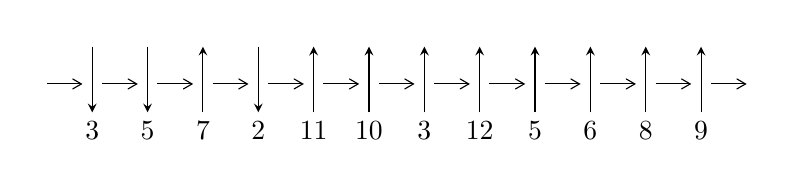
\begin{tikzpicture}[x=20pt, y=17pt]
	% nodes
	\node (C0) at (0, 0) {};
	\node (C1) at (1, 0) {};
	\node (C1U) at (1, +1) {};
	\node (C1D) at (1, -1) {3};

	\node (C2) at (2, 0) {};
	\node (C2U) at (2, +1) {};
	\node (C2D) at (2, -1) {5};

	\node (C3) at (3, 0) {};
	\node (C3U) at (3, +1) {};
	\node (C3D) at (3, -1) {7};

	\node (C4) at (4, 0) {};
	\node (C4U) at (4, +1) {};
	\node (C4D) at (4, -1) {2};

	\node (C5) at (5, 0) {};
	\node (C5U) at (5, +1) {};
	\node (C5D) at (5, -1) {11};

	\node (C6) at (6, 0) {};
	\node (C6U) at (6, +1) {};
	\node (C6D) at (6, -1) {10};

	\node (C7) at (7, 0) {};
	\node (C7U) at (7, +1) {};
	\node (C7D) at (7, -1) {3};

	\node (C8) at (8, 0) {};
	\node (C8U) at (8, +1) {};
	\node (C8D) at (8, -1) {12};

	\node (C9) at (9, 0) {};
	\node (C9U) at (9, +1) {};
	\node (C9D) at (9, -1) {5};

	\node (C10) at (10, 0) {};
	\node (C10U) at (10, +1) {};
	\node (C10D) at (10, -1) {6};

	\node (C11) at (11, 0) {};
	\node (C11U) at (11, +1) {};
	\node (C11D) at (11, -1) {8};

	\node (C12) at (12, 0) {};
	\node (C12U) at (12, +1) {};
	\node (C12D) at (12, -1) {9};
	\node (C13) at (13, 0) {};

	% arrows
	\draw[->,>={angle 60}]
	(C0) edge (C1) (C1) edge (C2) (C2) edge (C3) (C3) edge (C4) (C4) edge (C5) (C5) edge (C6) (C6) edge (C7) (C7) edge (C8) (C8) edge (C9) (C9) edge (C10) (C10) edge (C11) (C11) edge (C12) (C12) edge (C13) ;	\draw[->,>=stealth]
	(C1U) edge (C1D) (C2U) edge (C2D) (C3D) edge (C3U) (C4U) edge (C4D) (C5D) edge (C5U) (C6D) edge (C6U) (C7D) edge (C7U) (C8D) edge (C8U) (C9D) edge (C9U) (C10D) edge (C10U) (C11D) edge (C11U) (C12D) edge (C12U) ;
	\end{tikzpicture} \\
\hhline{~~} \\& 
\textbf{Solving Sequence} \\ \cline{2-2} 
 &
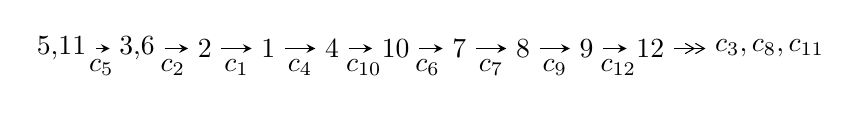
\begin{tikzpicture}[x=23pt, y=7pt]
	% node
	\node (A0) at (-1/8, 0) {5,11};
	\node (A1) at (17/16, 0) {3,6};
	\node (A2) at (17/8, 0) {2};
	\node (A3) at (25/8, 0) {1};
	\node (A4) at (33/8, 0) {4};
	\node (A5) at (41/8, 0) {10};
	\node (A6) at (49/8, 0) {7};
	\node (A7) at (57/8, 0) {8};
	\node (A8) at (65/8, 0) {9};
	\node (A9) at (73/8, 0) {12};
	\node (C1) at (1/2, -1) {$c_{5}$};
	\node (C2) at (13/8, -1) {$c_{2}$};
	\node (C3) at (21/8, -1) {$c_{1}$};
	\node (C4) at (29/8, -1) {$c_{4}$};
	\node (C5) at (37/8, -1) {$c_{10}$};
	\node (C6) at (45/8, -1) {$c_{6}$};
	\node (C7) at (53/8, -1) {$c_{7}$};
	\node (C8) at (61/8, -1) {$c_{9}$};
	\node (C9) at (69/8, -1) {$c_{12}$};
	\node (A10) at (11, 0) {$c_{3},c_{8},c_{11}$};

	% edge
	\draw[->,>=stealth]	
	(A0) edge (A1) (A1) edge (A2) (A2) edge (A3) (A3) edge (A4) (A4) edge (A5) (A5) edge (A6) (A6) edge (A7) (A7) edge (A8) (A8) edge (A9) ;
	\draw[->>,>={angle 60}]	
	(A9) edge (A10);
\end{tikzpicture} \\ 

\end{tabular} \\

\footnotetext{
The image of knot diagram is generated by the software ``\textbf{Draw programme}" developed by Andrew Bartholomew(\url{http://www.layer8.co.uk/maths/draw/index.htm\#Running-draw}), where we modified some parts for our purpose(\url{https://github.com/CATsTAILs/LinksPainter}).
}\phantom \\ \newline 
\centering \textbf{Ideals for irreducible components\footnotemark of $X_{\text{par}}$} 
 
\begin{align*}
I^u_{1}&=\langle 
-3.03075\times10^{15} u^{34}+5.04695\times10^{15} u^{33}+\cdots+8.13080\times10^{15} b+2.21604\times10^{15},\\
\phantom{I^u_{1}}&\phantom{= \langle  }2.79762\times10^{15} u^{34}-1.92144\times10^{15} u^{33}+\cdots+2.43924\times10^{16} a-5.33582\times10^{16},\;u^{35}-2 u^{34}+\cdots+2 u-1\rangle \\
I^u_{2}&=\langle 
b+1,\;2 u^5-4 u^4+7 u^3-8 u^2+3 a+6 u-5,\;u^6- u^5+3 u^4-2 u^3+2 u^2- u-1\rangle \\
\\
\end{align*}
\raggedright * 2 irreducible components of $\dim_{\mathbb{C}}=0$, with total 41 representations.\\
\footnotetext{All coefficients of polynomials are rational numbers. But the coefficients are sometimes approximated in decimal forms when there is not enough margin.}
\newpage
\renewcommand{\arraystretch}{1}
\centering \section*{I. $I^u_{1}= \langle -3.03\times10^{15} u^{34}+5.05\times10^{15} u^{33}+\cdots+8.13\times10^{15} b+2.22\times10^{15},\;2.80\times10^{15} u^{34}-1.92\times10^{15} u^{33}+\cdots+2.44\times10^{16} a-5.34\times10^{16},\;u^{35}-2 u^{34}+\cdots+2 u-1 \rangle$}
\flushleft \textbf{(i) Arc colorings}\\
\begin{tabular}{m{7pt} m{180pt} m{7pt} m{180pt} }
\flushright $a_{5}=$&$\begin{pmatrix}1\\0\end{pmatrix}$ \\
\flushright $a_{11}=$&$\begin{pmatrix}0\\u\end{pmatrix}$ \\
\flushright $a_{3}=$&$\begin{pmatrix}-0.114692 u^{34}+0.0787722 u^{33}+\cdots-1.96825 u+2.18749\\0.372749 u^{34}-0.620720 u^{33}+\cdots-0.234090 u-0.272549\end{pmatrix}$ \\
\flushright $a_{6}=$&$\begin{pmatrix}1\\- u^2\end{pmatrix}$ \\
\flushright $a_{2}=$&$\begin{pmatrix}0.258057 u^{34}-0.541948 u^{33}+\cdots-2.20234 u+1.91494\\0.372749 u^{34}-0.620720 u^{33}+\cdots-0.234090 u-0.272549\end{pmatrix}$ \\
\flushright $a_{1}=$&$\begin{pmatrix}0.690547 u^{34}-1.46587 u^{33}+\cdots+0.955473 u+1.23197\\0.155004 u^{34}-0.146233 u^{33}+\cdots-0.509081 u+0.0465323\end{pmatrix}$ \\
\flushright $a_{4}=$&$\begin{pmatrix}-0.163208 u^{34}+0.206889 u^{33}+\cdots-2.24117 u+1.89622\\0.309999 u^{34}-0.565156 u^{33}+\cdots-0.0329643 u-0.311311\end{pmatrix}$ \\
\flushright $a_{10}=$&$\begin{pmatrix}- u\\u^3+u\end{pmatrix}$ \\
\flushright $a_{7}=$&$\begin{pmatrix}u^2+1\\- u^4-2 u^2\end{pmatrix}$ \\
\flushright $a_{8}=$&$\begin{pmatrix}0.975045 u^{34}-1.56629 u^{33}+\cdots+0.624872 u+1.40403\\-0.178130 u^{34}+0.294487 u^{33}+\cdots-0.385935 u-0.509322\end{pmatrix}$ \\
\flushright $a_{9}=$&$\begin{pmatrix}- u^3-2 u\\u^3+u\end{pmatrix}$ \\
\flushright $a_{12}=$&$\begin{pmatrix}0.731265 u^{34}-1.31399 u^{33}+\cdots+0.00587251 u+0.707409\\0.0656504 u^{34}+0.0421843 u^{33}+\cdots+0.233065 u+0.187300\end{pmatrix}$\\&\end{tabular}
\flushleft \textbf{(ii) Obstruction class $= -1$}\\~\\
\flushleft \textbf{(iii) Cusp Shapes $= \frac{103503859831926074}{73177204311856557} u^{34}-\frac{16140270790780718}{8130800479095173} u^{33}+\cdots-\frac{152451832308656366}{24392401437285519} u+\frac{913459447845182116}{73177204311856557}$}\\~\\
\newpage\renewcommand{\arraystretch}{1}
\flushleft \textbf{(iv) u-Polynomials at the component}\newline \\
\begin{tabular}{m{50pt}|m{274pt}}
Crossings & \hspace{64pt}u-Polynomials at each crossing \\
\hline $$\begin{aligned}c_{1}\end{aligned}$$&$\begin{aligned}
&u^{35}+43 u^{34}+\cdots+12249 u+81
\end{aligned}$\\
\hline $$\begin{aligned}c_{2},c_{4}\end{aligned}$$&$\begin{aligned}
&u^{35}-7 u^{34}+\cdots-129 u+9
\end{aligned}$\\
\hline $$\begin{aligned}c_{3},c_{7}\end{aligned}$$&$\begin{aligned}
&u^{35}-3 u^{34}+\cdots+192 u-576
\end{aligned}$\\
\hline $$\begin{aligned}c_{5},c_{6},c_{10}\end{aligned}$$&$\begin{aligned}
&u^{35}-2 u^{34}+\cdots+2 u-1
\end{aligned}$\\
\hline $$\begin{aligned}c_{8},c_{11},c_{12}\end{aligned}$$&$\begin{aligned}
&u^{35}-2 u^{34}+\cdots-2 u+1
\end{aligned}$\\
\hline $$\begin{aligned}c_{9}\end{aligned}$$&$\begin{aligned}
&u^{35}+2 u^{34}+\cdots+150 u-1697
\end{aligned}$\\
\hline
\end{tabular}\\~\\
\newpage\renewcommand{\arraystretch}{1}
\flushleft \textbf{(v) Riley Polynomials at the component}\newline \\
\begin{tabular}{m{50pt}|m{274pt}}
Crossings & \hspace{64pt}Riley Polynomials at each crossing \\
\hline $$\begin{aligned}c_{1}\end{aligned}$$&$\begin{aligned}
&y^{35}-95 y^{34}+\cdots+108831357 y-6561
\end{aligned}$\\
\hline $$\begin{aligned}c_{2},c_{4}\end{aligned}$$&$\begin{aligned}
&y^{35}-43 y^{34}+\cdots+12249 y-81
\end{aligned}$\\
\hline $$\begin{aligned}c_{3},c_{7}\end{aligned}$$&$\begin{aligned}
&y^{35}+39 y^{34}+\cdots+4349952 y-331776
\end{aligned}$\\
\hline $$\begin{aligned}c_{5},c_{6},c_{10}\end{aligned}$$&$\begin{aligned}
&y^{35}+36 y^{34}+\cdots+4 y-1
\end{aligned}$\\
\hline $$\begin{aligned}c_{8},c_{11},c_{12}\end{aligned}$$&$\begin{aligned}
&y^{35}-24 y^{34}+\cdots+4 y-1
\end{aligned}$\\
\hline $$\begin{aligned}c_{9}\end{aligned}$$&$\begin{aligned}
&y^{35}+36 y^{34}+\cdots-44085924 y-2879809
\end{aligned}$\\
\hline
\end{tabular}\\~\\
\newpage\flushleft \textbf{(vi) Complex Volumes and Cusp Shapes}
$$\begin{array}{c|c|c}  
\text{Solutions to }I^u_{1}& \I (\text{vol} + \sqrt{-1}CS) & \text{Cusp shape}\\
 \hline 
\begin{aligned}
u &= \phantom{-}0.808354 + 0.590795 I \\
a &= -0.96671 + 1.32263 I \\
b &= \phantom{-}1.60615 - 0.32627 I\end{aligned}
 & -6.00623 + 8.79867 I & \phantom{-}4.77908 - 5.93735 I \\ \hline\begin{aligned}
u &= \phantom{-}0.808354 - 0.590795 I \\
a &= -0.96671 - 1.32263 I \\
b &= \phantom{-}1.60615 + 0.32627 I\end{aligned}
 & -6.00623 - 8.79867 I & \phantom{-}4.77908 + 5.93735 I \\ \hline\begin{aligned}
u &= \phantom{-}0.842677 + 0.549259 I \\
a &= -1.27004 + 0.62262 I \\
b &= \phantom{-}1.58817 + 0.14912 I\end{aligned}
 & -5.85440 - 3.32055 I & \phantom{-}4.34747 + 0.93966 I \\ \hline\begin{aligned}
u &= \phantom{-}0.842677 - 0.549259 I \\
a &= -1.27004 - 0.62262 I \\
b &= \phantom{-}1.58817 - 0.14912 I\end{aligned}
 & -5.85440 + 3.32055 I & \phantom{-}4.34747 - 0.93966 I \\ \hline\begin{aligned}
u &= -0.827360 + 0.573264 I \\
a &= -1.20940 - 1.01711 I \\
b &= \phantom{-}1.66577 + 0.09214 I\end{aligned}
 & -10.19960 - 2.74879 I & \phantom{-}1.97037 + 2.55405 I \\ \hline\begin{aligned}
u &= -0.827360 - 0.573264 I \\
a &= -1.20940 + 1.01711 I \\
b &= \phantom{-}1.66577 - 0.09214 I\end{aligned}
 & -10.19960 + 2.74879 I & \phantom{-}1.97037 - 2.55405 I \\ \hline\begin{aligned}
u &= -0.811473\phantom{ +0.000000I} \\
a &= -0.265837\phantom{ +0.000000I} \\
b &= \phantom{-}0.650017\phantom{ +0.000000I}\end{aligned}
 & \phantom{-}6.62664\phantom{ +0.000000I} & \phantom{-}17.6690\phantom{ +0.000000I} \\ \hline\begin{aligned}
u &= \phantom{-}0.107218 + 1.291980 I \\
a &= \phantom{-}0.434714 - 0.101824 I \\
b &= \phantom{-}0.264007 + 0.190902 I\end{aligned}
 & -3.34436 + 1.70345 I & \phantom{-}6.00000 - 3.39166 I \\ \hline\begin{aligned}
u &= \phantom{-}0.107218 - 1.291980 I \\
a &= \phantom{-}0.434714 + 0.101824 I \\
b &= \phantom{-}0.264007 - 0.190902 I\end{aligned}
 & -3.34436 - 1.70345 I & \phantom{-}6.00000 + 3.39166 I \\ \hline\begin{aligned}
u &= -0.351791 + 1.294310 I \\
a &= \phantom{-}0.169982 - 0.171072 I \\
b &= \phantom{-}0.703358 - 0.244061 I\end{aligned}
 & \phantom{-}2.59761 - 4.19287 I & \phantom{-}11.68502 + 0. I\phantom{ +0.000000I}\\
 \hline 
 \end{array}$$\newpage$$\begin{array}{c|c|c}  
\text{Solutions to }I^u_{1}& \I (\text{vol} + \sqrt{-1}CS) & \text{Cusp shape}\\
 \hline 
\begin{aligned}
u &= -0.351791 - 1.294310 I \\
a &= \phantom{-}0.169982 + 0.171072 I \\
b &= \phantom{-}0.703358 + 0.244061 I\end{aligned}
 & \phantom{-}2.59761 + 4.19287 I & \phantom{-}11.68502 + 0. I\phantom{ +0.000000I} \\ \hline\begin{aligned}
u &= \phantom{-}0.442125 + 0.465797 I \\
a &= \phantom{-}0.29153 - 1.72600 I \\
b &= -0.450029 + 0.982563 I\end{aligned}
 & \phantom{-}0.85715 + 4.05468 I & \phantom{-}7.07282 - 8.26213 I \\ \hline\begin{aligned}
u &= \phantom{-}0.442125 - 0.465797 I \\
a &= \phantom{-}0.29153 + 1.72600 I \\
b &= -0.450029 - 0.982563 I\end{aligned}
 & \phantom{-}0.85715 - 4.05468 I & \phantom{-}7.07282 + 8.26213 I \\ \hline\begin{aligned}
u &= \phantom{-}0.06324 + 1.42930 I \\
a &= \phantom{-}0.79947 - 1.80755 I \\
b &= -0.669626 + 0.122395 I\end{aligned}
 & -4.33630 + 0.24126 I & \phantom{-0.000000 -}0. + 2.29622 I \\ \hline\begin{aligned}
u &= \phantom{-}0.06324 - 1.42930 I \\
a &= \phantom{-}0.79947 + 1.80755 I \\
b &= -0.669626 - 0.122395 I\end{aligned}
 & -4.33630 - 0.24126 I & \phantom{-0.000000 } 0. - 2.29622 I \\ \hline\begin{aligned}
u &= -0.119731 + 0.541272 I \\
a &= \phantom{-}0.540705 + 0.927189 I \\
b &= -1.384480 - 0.284252 I\end{aligned}
 & -2.19113 - 1.44339 I & \phantom{-}0.79876 + 4.24276 I \\ \hline\begin{aligned}
u &= -0.119731 - 0.541272 I \\
a &= \phantom{-}0.540705 - 0.927189 I \\
b &= -1.384480 + 0.284252 I\end{aligned}
 & -2.19113 + 1.44339 I & \phantom{-}0.79876 - 4.24276 I \\ \hline\begin{aligned}
u &= \phantom{-}0.390353 + 0.322694 I \\
a &= \phantom{-}2.47912 - 0.17252 I \\
b &= -0.426347 - 0.408392 I\end{aligned}
 & \phantom{-}1.15302 - 1.16635 I & \phantom{-}8.59535 - 1.69076 I \\ \hline\begin{aligned}
u &= \phantom{-}0.390353 - 0.322694 I \\
a &= \phantom{-}2.47912 + 0.17252 I \\
b &= -0.426347 + 0.408392 I\end{aligned}
 & \phantom{-}1.15302 + 1.16635 I & \phantom{-}8.59535 + 1.69076 I \\ \hline\begin{aligned}
u &= -0.07785 + 1.49505 I \\
a &= -0.283980 + 0.919506 I \\
b &= -1.056680 - 0.871979 I\end{aligned}
 & -7.88732 - 2.21831 I & \phantom{-0.000000 } 0\\
 \hline 
 \end{array}$$\newpage$$\begin{array}{c|c|c}  
\text{Solutions to }I^u_{1}& \I (\text{vol} + \sqrt{-1}CS) & \text{Cusp shape}\\
 \hline 
\begin{aligned}
u &= -0.07785 - 1.49505 I \\
a &= -0.283980 - 0.919506 I \\
b &= -1.056680 + 0.871979 I\end{aligned}
 & -7.88732 + 2.21831 I & \phantom{-0.000000 } 0 \\ \hline\begin{aligned}
u &= \phantom{-}0.12308 + 1.50667 I \\
a &= -0.255885 - 0.817683 I \\
b &= -0.62821 + 1.42265 I\end{aligned}
 & -5.67256 + 6.05068 I & \phantom{-0.000000 } 0 \\ \hline\begin{aligned}
u &= \phantom{-}0.12308 - 1.50667 I \\
a &= -0.255885 + 0.817683 I \\
b &= -0.62821 - 1.42265 I\end{aligned}
 & -5.67256 - 6.05068 I & \phantom{-0.000000 } 0 \\ \hline\begin{aligned}
u &= -0.285882 + 0.388697 I \\
a &= \phantom{-}0.71032 + 1.88285 I \\
b &= -0.794496 - 0.374564 I\end{aligned}
 & -1.59088 - 0.96138 I & -0.24473 + 3.68390 I \\ \hline\begin{aligned}
u &= -0.285882 - 0.388697 I \\
a &= \phantom{-}0.71032 - 1.88285 I \\
b &= -0.794496 + 0.374564 I\end{aligned}
 & -1.59088 + 0.96138 I & -0.24473 - 3.68390 I \\ \hline\begin{aligned}
u &= -0.02272 + 1.52580 I \\
a &= -0.366013 + 0.335128 I \\
b &= -1.84971 - 0.36801 I\end{aligned}
 & -9.09046 - 1.89171 I & \phantom{-0.000000 } 0 \\ \hline\begin{aligned}
u &= -0.02272 - 1.52580 I \\
a &= -0.366013 - 0.335128 I \\
b &= -1.84971 + 0.36801 I\end{aligned}
 & -9.09046 + 1.89171 I & \phantom{-0.000000 } 0 \\ \hline\begin{aligned}
u &= \phantom{-}0.27448 + 1.56892 I \\
a &= \phantom{-}0.243584 + 1.215400 I \\
b &= \phantom{-}1.69785 - 0.47016 I\end{aligned}
 & -13.0918 + 12.7942 I & \phantom{-0.000000 } 0 \\ \hline\begin{aligned}
u &= \phantom{-}0.27448 - 1.56892 I \\
a &= \phantom{-}0.243584 - 1.215400 I \\
b &= \phantom{-}1.69785 + 0.47016 I\end{aligned}
 & -13.0918 - 12.7942 I & \phantom{-0.000000 } 0 \\ \hline\begin{aligned}
u &= -0.28497 + 1.57001 I \\
a &= \phantom{-}0.066691 - 1.110120 I \\
b &= \phantom{-}1.75299 + 0.26356 I\end{aligned}
 & -17.2266 - 6.8599 I & \phantom{-0.000000 } 0\\
 \hline 
 \end{array}$$\newpage$$\begin{array}{c|c|c}  
\text{Solutions to }I^u_{1}& \I (\text{vol} + \sqrt{-1}CS) & \text{Cusp shape}\\
 \hline 
\begin{aligned}
u &= -0.28497 - 1.57001 I \\
a &= \phantom{-}0.066691 + 1.110120 I \\
b &= \phantom{-}1.75299 - 0.26356 I\end{aligned}
 & -17.2266 + 6.8599 I & \phantom{-0.000000 } 0 \\ \hline\begin{aligned}
u &= \phantom{-}0.29799 + 1.57077 I \\
a &= -0.034659 + 0.906346 I \\
b &= \phantom{-}1.66579 - 0.03532 I\end{aligned}
 & -12.79260 + 0.91123 I & \phantom{-0.000000 } 0 \\ \hline\begin{aligned}
u &= \phantom{-}0.29799 - 1.57077 I \\
a &= -0.034659 - 0.906346 I \\
b &= \phantom{-}1.66579 + 0.03532 I\end{aligned}
 & -12.79260 - 0.91123 I & \phantom{-0.000000 } 0 \\ \hline\begin{aligned}
u &= \phantom{-}0.388054\phantom{ +0.000000I} \\
a &= \phantom{-}0.599688\phantom{ +0.000000I} \\
b &= \phantom{-}0.0879256\phantom{ +0.000000I}\end{aligned}
 & \phantom{-}0.630605\phantom{ +0.000000I} & \phantom{-}15.9000\phantom{ +0.000000I} \\ \hline\begin{aligned}
u &= -0.335008\phantom{ +0.000000I} \\
a &= \phantom{-}7.30064\phantom{ +0.000000I} \\
b &= -1.10696\phantom{ +0.000000I}\end{aligned}
 & -0.492065\phantom{ +0.000000I} & \phantom{-}30.0890\phantom{ +0.000000I}\\
 \hline 
 \end{array}$$\newpage\newpage\renewcommand{\arraystretch}{1}
\centering \section*{II. $I^u_{2}= \langle b+1,\;2 u^5-4 u^4+7 u^3-8 u^2+3 a+6 u-5,\;u^6- u^5+3 u^4-2 u^3+2 u^2- u-1 \rangle$}
\flushleft \textbf{(i) Arc colorings}\\
\begin{tabular}{m{7pt} m{180pt} m{7pt} m{180pt} }
\flushright $a_{5}=$&$\begin{pmatrix}1\\0\end{pmatrix}$ \\
\flushright $a_{11}=$&$\begin{pmatrix}0\\u\end{pmatrix}$ \\
\flushright $a_{3}=$&$\begin{pmatrix}-\frac{2}{3} u^5+\frac{4}{3} u^4+\cdots-2 u+\frac{5}{3}\\-1\end{pmatrix}$ \\
\flushright $a_{6}=$&$\begin{pmatrix}1\\- u^2\end{pmatrix}$ \\
\flushright $a_{2}=$&$\begin{pmatrix}-\frac{2}{3} u^5+\frac{4}{3} u^4+\cdots-2 u+\frac{2}{3}\\-1\end{pmatrix}$ \\
\flushright $a_{1}=$&$\begin{pmatrix}-1\\0\end{pmatrix}$ \\
\flushright $a_{4}=$&$\begin{pmatrix}-\frac{2}{3} u^5+\frac{4}{3} u^4+\cdots-2 u+\frac{5}{3}\\-1\end{pmatrix}$ \\
\flushright $a_{10}=$&$\begin{pmatrix}- u\\u^3+u\end{pmatrix}$ \\
\flushright $a_{7}=$&$\begin{pmatrix}u^2+1\\- u^4-2 u^2\end{pmatrix}$ \\
\flushright $a_{8}=$&$\begin{pmatrix}u^2+1\\- u^4-2 u^2\end{pmatrix}$ \\
\flushright $a_{9}=$&$\begin{pmatrix}- u^3-2 u\\u^3+u\end{pmatrix}$ \\
\flushright $a_{12}=$&$\begin{pmatrix}u^5+2 u^3+u\\- u^5+u^4-2 u^3+u^2- u-1\end{pmatrix}$\\&\end{tabular}
\flushleft \textbf{(ii) Obstruction class $= 1$}\\~\\
\flushleft \textbf{(iii) Cusp Shapes $= \frac{7}{9} u^5+\frac{31}{9} u^4-\frac{10}{9} u^3+\frac{41}{9} u^2-2 u+\frac{2}{9}$}\\~\\
\newpage\renewcommand{\arraystretch}{1}
\flushleft \textbf{(iv) u-Polynomials at the component}\newline \\
\begin{tabular}{m{50pt}|m{274pt}}
Crossings & \hspace{64pt}u-Polynomials at each crossing \\
\hline $$\begin{aligned}c_{1},c_{2}\end{aligned}$$&$\begin{aligned}
&(u-1)^6
\end{aligned}$\\
\hline $$\begin{aligned}c_{3},c_{7}\end{aligned}$$&$\begin{aligned}
&u^6
\end{aligned}$\\
\hline $$\begin{aligned}c_{4}\end{aligned}$$&$\begin{aligned}
&(u+1)^6
\end{aligned}$\\
\hline $$\begin{aligned}c_{5},c_{6}\end{aligned}$$&$\begin{aligned}
&u^6- u^5+3 u^4-2 u^3+2 u^2- u-1
\end{aligned}$\\
\hline $$\begin{aligned}c_{8}\end{aligned}$$&$\begin{aligned}
&u^6+u^5-3 u^4-2 u^3+2 u^2- u-1
\end{aligned}$\\
\hline $$\begin{aligned}c_{9},c_{11},c_{12}\end{aligned}$$&$\begin{aligned}
&u^6- u^5-3 u^4+2 u^3+2 u^2+u-1
\end{aligned}$\\
\hline $$\begin{aligned}c_{10}\end{aligned}$$&$\begin{aligned}
&u^6+u^5+3 u^4+2 u^3+2 u^2+u-1
\end{aligned}$\\
\hline
\end{tabular}\\~\\
\newpage\renewcommand{\arraystretch}{1}
\flushleft \textbf{(v) Riley Polynomials at the component}\newline \\
\begin{tabular}{m{50pt}|m{274pt}}
Crossings & \hspace{64pt}Riley Polynomials at each crossing \\
\hline $$\begin{aligned}c_{1},c_{2},c_{4}\end{aligned}$$&$\begin{aligned}
&(y-1)^6
\end{aligned}$\\
\hline $$\begin{aligned}c_{3},c_{7}\end{aligned}$$&$\begin{aligned}
&y^6
\end{aligned}$\\
\hline $$\begin{aligned}c_{5},c_{6},c_{10}\end{aligned}$$&$\begin{aligned}
&y^6+5 y^5+9 y^4+4 y^3-6 y^2-5 y+1
\end{aligned}$\\
\hline $$\begin{aligned}c_{8},c_{9},c_{11}\\c_{12}\end{aligned}$$&$\begin{aligned}
&y^6-7 y^5+17 y^4-16 y^3+6 y^2-5 y+1
\end{aligned}$\\
\hline
\end{tabular}\\~\\
\newpage\flushleft \textbf{(vi) Complex Volumes and Cusp Shapes}
$$\begin{array}{c|c|c}  
\text{Solutions to }I^u_{2}& \I (\text{vol} + \sqrt{-1}CS) & \text{Cusp shape}\\
 \hline 
\begin{aligned}
u &= \phantom{-}0.873214\phantom{ +0.000000I} \\
a &= \phantom{-}0.836730\phantom{ +0.000000I} \\
b &= -1.00000\phantom{ +0.000000I}\end{aligned}
 & \phantom{-}6.01515\phantom{ +0.000000I} & \phantom{-}3.60710\phantom{ +0.000000I} \\ \hline\begin{aligned}
u &= -0.138835 + 1.234450 I \\
a &= \phantom{-}0.366605 + 0.544193 I \\
b &= -1.00000\phantom{ +0.000000I}\end{aligned}
 & -4.60518 - 1.97241 I & -0.88590 + 3.48248 I \\ \hline\begin{aligned}
u &= -0.138835 - 1.234450 I \\
a &= \phantom{-}0.366605 - 0.544193 I \\
b &= -1.00000\phantom{ +0.000000I}\end{aligned}
 & -4.60518 + 1.97241 I & -0.88590 - 3.48248 I \\ \hline\begin{aligned}
u &= \phantom{-}0.408802 + 1.276380 I \\
a &= -0.031424 - 0.540243 I \\
b &= -1.00000\phantom{ +0.000000I}\end{aligned}
 & \phantom{-}2.05064 + 4.59213 I & \phantom{-}1.86238 - 6.63921 I \\ \hline\begin{aligned}
u &= \phantom{-}0.408802 - 1.276380 I \\
a &= -0.031424 + 0.540243 I \\
b &= -1.00000\phantom{ +0.000000I}\end{aligned}
 & \phantom{-}2.05064 - 4.59213 I & \phantom{-}1.86238 + 6.63921 I \\ \hline\begin{aligned}
u &= -0.413150\phantom{ +0.000000I} \\
a &= \phantom{-}3.15957\phantom{ +0.000000I} \\
b &= -1.00000\phantom{ +0.000000I}\end{aligned}
 & -0.906083\phantom{ +0.000000I} & \phantom{-}1.99550\phantom{ +0.000000I}\\
 \hline 
 \end{array}$$\newpage
\newpage\renewcommand{\arraystretch}{1}
\centering \section*{ III. u-Polynomials}
\begin{tabular}{m{50pt}|m{274pt}}
Crossings & \hspace{64pt}u-Polynomials at each crossing \\
\hline $$\begin{aligned}c_{1}\end{aligned}$$&$\begin{aligned}
&((u-1)^6)(u^{35}+43 u^{34}+\cdots+12249 u+81)
\end{aligned}$\\
\hline $$\begin{aligned}c_{2}\end{aligned}$$&$\begin{aligned}
&((u-1)^6)(u^{35}-7 u^{34}+\cdots-129 u+9)
\end{aligned}$\\
\hline $$\begin{aligned}c_{3},c_{7}\end{aligned}$$&$\begin{aligned}
&u^6(u^{35}-3 u^{34}+\cdots+192 u-576)
\end{aligned}$\\
\hline $$\begin{aligned}c_{4}\end{aligned}$$&$\begin{aligned}
&((u+1)^6)(u^{35}-7 u^{34}+\cdots-129 u+9)
\end{aligned}$\\
\hline $$\begin{aligned}c_{5},c_{6}\end{aligned}$$&$\begin{aligned}
&(u^6- u^5+3 u^4-2 u^3+2 u^2- u-1)(u^{35}-2 u^{34}+\cdots+2 u-1)
\end{aligned}$\\
\hline $$\begin{aligned}c_{8}\end{aligned}$$&$\begin{aligned}
&(u^6+u^5-3 u^4-2 u^3+2 u^2- u-1)(u^{35}-2 u^{34}+\cdots-2 u+1)
\end{aligned}$\\
\hline $$\begin{aligned}c_{9}\end{aligned}$$&$\begin{aligned}
&(u^6- u^5-3 u^4+2 u^3+2 u^2+u-1)(u^{35}+2 u^{34}+\cdots+150 u-1697)
\end{aligned}$\\
\hline $$\begin{aligned}c_{10}\end{aligned}$$&$\begin{aligned}
&(u^6+u^5+3 u^4+2 u^3+2 u^2+u-1)(u^{35}-2 u^{34}+\cdots+2 u-1)
\end{aligned}$\\
\hline $$\begin{aligned}c_{11},c_{12}\end{aligned}$$&$\begin{aligned}
&(u^6- u^5-3 u^4+2 u^3+2 u^2+u-1)(u^{35}-2 u^{34}+\cdots-2 u+1)
\end{aligned}$\\
\hline
\end{tabular}\newpage\renewcommand{\arraystretch}{1}
\centering \section*{ IV. Riley Polynomials}
\begin{tabular}{m{50pt}|m{274pt}}
Crossings & \hspace{64pt}Riley Polynomials at each crossing \\
\hline $$\begin{aligned}c_{1}\end{aligned}$$&$\begin{aligned}
&((y-1)^6)(y^{35}-95 y^{34}+\cdots+1.08831\times10^{8} y-6561)
\end{aligned}$\\
\hline $$\begin{aligned}c_{2},c_{4}\end{aligned}$$&$\begin{aligned}
&((y-1)^6)(y^{35}-43 y^{34}+\cdots+12249 y-81)
\end{aligned}$\\
\hline $$\begin{aligned}c_{3},c_{7}\end{aligned}$$&$\begin{aligned}
&y^6(y^{35}+39 y^{34}+\cdots+4349952 y-331776)
\end{aligned}$\\
\hline $$\begin{aligned}c_{5},c_{6},c_{10}\end{aligned}$$&$\begin{aligned}
&(y^6+5 y^5+\cdots-5 y+1)(y^{35}+36 y^{34}+\cdots+4 y-1)
\end{aligned}$\\
\hline $$\begin{aligned}c_{8},c_{11},c_{12}\end{aligned}$$&$\begin{aligned}
&(y^6-7 y^5+\cdots-5 y+1)(y^{35}-24 y^{34}+\cdots+4 y-1)
\end{aligned}$\\
\hline $$\begin{aligned}c_{9}\end{aligned}$$&$\begin{aligned}
&(y^6-7 y^5+17 y^4-16 y^3+6 y^2-5 y+1)\\
&\cdot(y^{35}+36 y^{34}+\cdots-44085924 y-2879809)
\end{aligned}$\\
\hline
\end{tabular}
\vskip 2pc
\end{document}